%caro
\begin{figure}
\caption{Figures from Caro (1995) demonstrating the development of play behavior in cheetah cubs.}
  \begin{center}
    \begin{minipage}[t]{0.48\linewidth}
      a)\\
      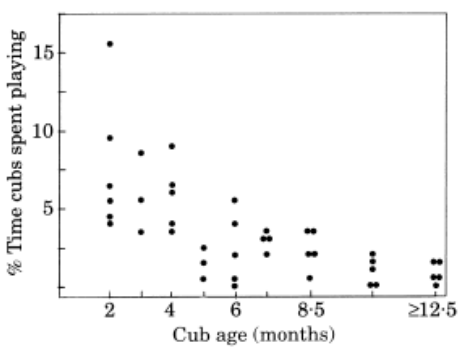
\includegraphics[width=83mm]{caroFig1edit.png}\\
      b)\\
      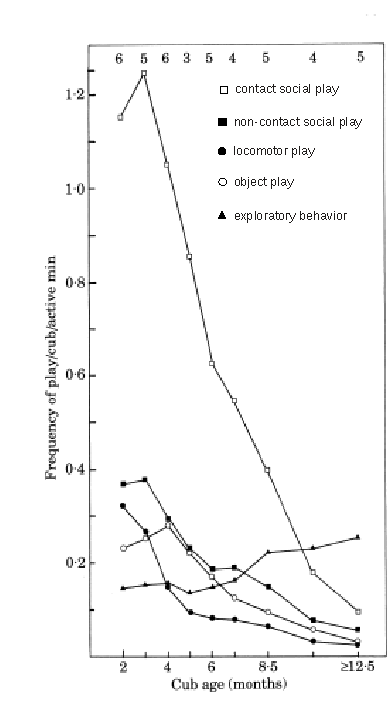
\includegraphics[width=80mm]{caroFig2edit.pdf}
    \end{minipage}\hfill
    \begin{minipage}[t]{0.48\linewidth}
       \\\\a) The average percentage of time spent playing in 15 minute observations. 41 litters were observed. Each point represents an average for each litter. Total play decreases as cheetahs get older. 
       \\\\\\\\\\\\\\\\\\\\\\b) Running mean values of indicated play types. Number of litters from each age class shown across the top. Displayed play type changes with age, all types of social play decrease with age, while exploratory behavior increases with age. 
    \end{minipage}
  \end{center}
\end{figure}



%skill development line
\begin{figure}[h]
\caption{A representation of the development of play behavior with respect to the model. In the terminal condition ($t=T$), $\phi(i)$ is defined based on the life history of the modeled organism for all time periods beyond $T$. The model is solved backwards in time to yield fitness values for every period of the model, $F(i,t)$, as well as play decisions for ever period of the model, $D^*(i,j,t)$.}
\begin{center}
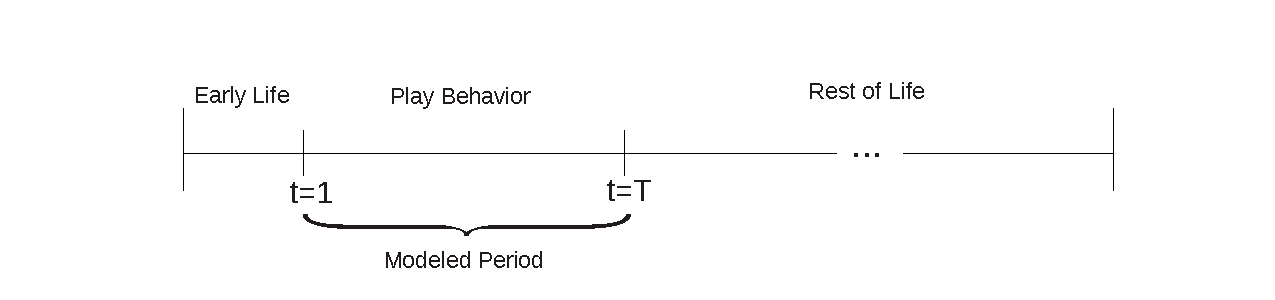
\includegraphics[width=170mm]{numberLineOfLife.pdf}
\end{center}
\label{sdf}
\end{figure}



%bell curve with Alpha Tau
\begin{figure}[h]
\caption{$\Delta S(i,j)$. The skill increment function showing several values of $\sigma$. $\Delta S(i,j)$ is plotted alongside the skill decrement $\alpha \tau$. Myopic focal individuals play with any play partner such that $i-j$ causes $\Delta S(i,j)>\alpha \tau$. Notice as $\sigma$ increases the range of potential play partners increases. For the optimal focal individual the play threshold lies some distance above $\alpha \tau$ based on the focal individuals skill and the amount of time remaining in the model.      }
\begin{center}
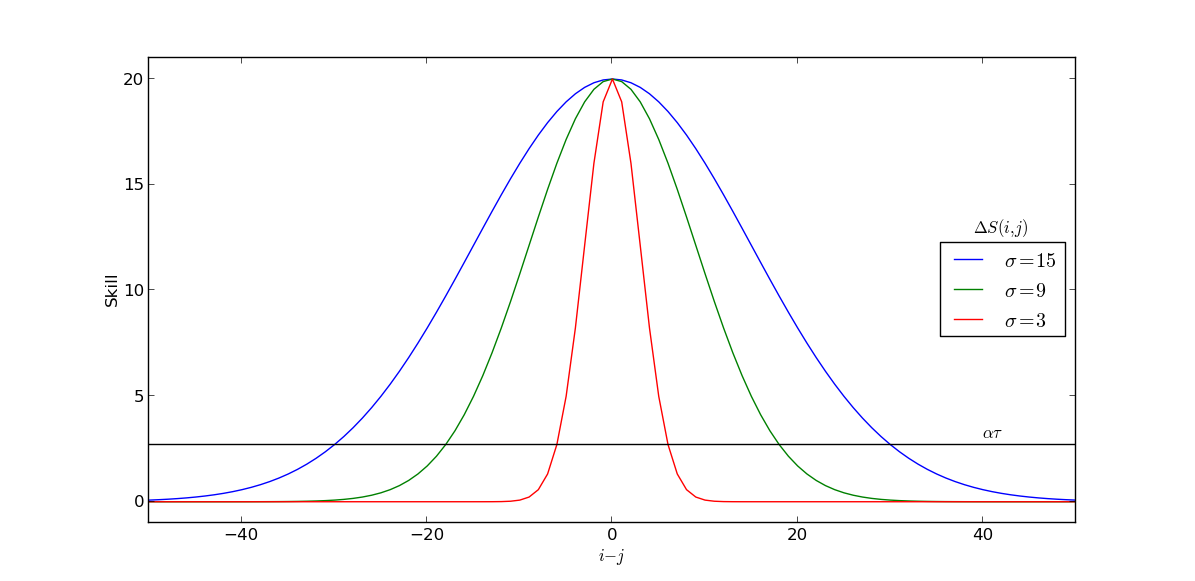
\includegraphics[width=160mm]{sdf.png}
\end{center}
\label{sdf}
\end{figure}



%future fitness
\begin{figure}[h]
\caption{$\phi(i)$. Three possible trajectories for $\phi(i)$. Notice the greater the steepness parameter $\gamma$ the more quickly and dramatically the organism matures once it reaches adolescence. }
\begin{center}
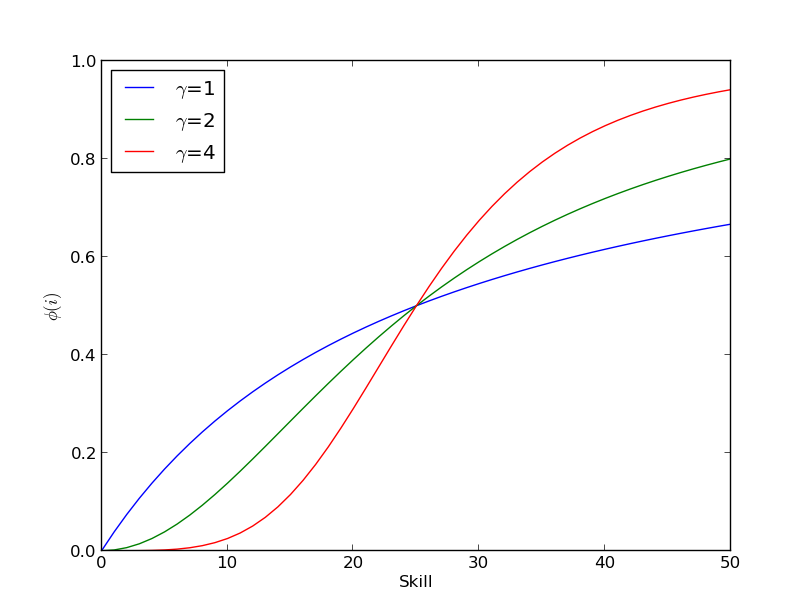
\includegraphics[width=160mm]{phi.png}
\end{center}
\label{phi}
\end{figure}



%heatmap
\begin{figure}[h]
\caption{$R(i,t)$. A grey scale representation of the focal individual play range as a function of both time and focal individual skill level. Dark cells are representative of focal individuals willing to play with play partners of many different skill levels, while light cells are representative of focal individuals with relatively small play ranges. In general as skill increases focal individual play range increases. Additionally as $t$ approaches $T$, in general, play range increases to the myopic condition, at $T-1$. However, a pocket of lower than expected play ranges does violate these general trends. This pocket occurs at relatively high values for $t$ and extends across all of the playing skill levels. This pocket is produced by truncating play events as $t$ approaches $T$. }%  .The complex patterns occurring at time periods just prior to $T-1$, at low skills, and time periods just prior to exiting, for high skills, are the effects of truncating of play events as $t$ approaches $T$.   }
\begin{center}
%\includegraphics[width=150mm]{playOpportunites.png}
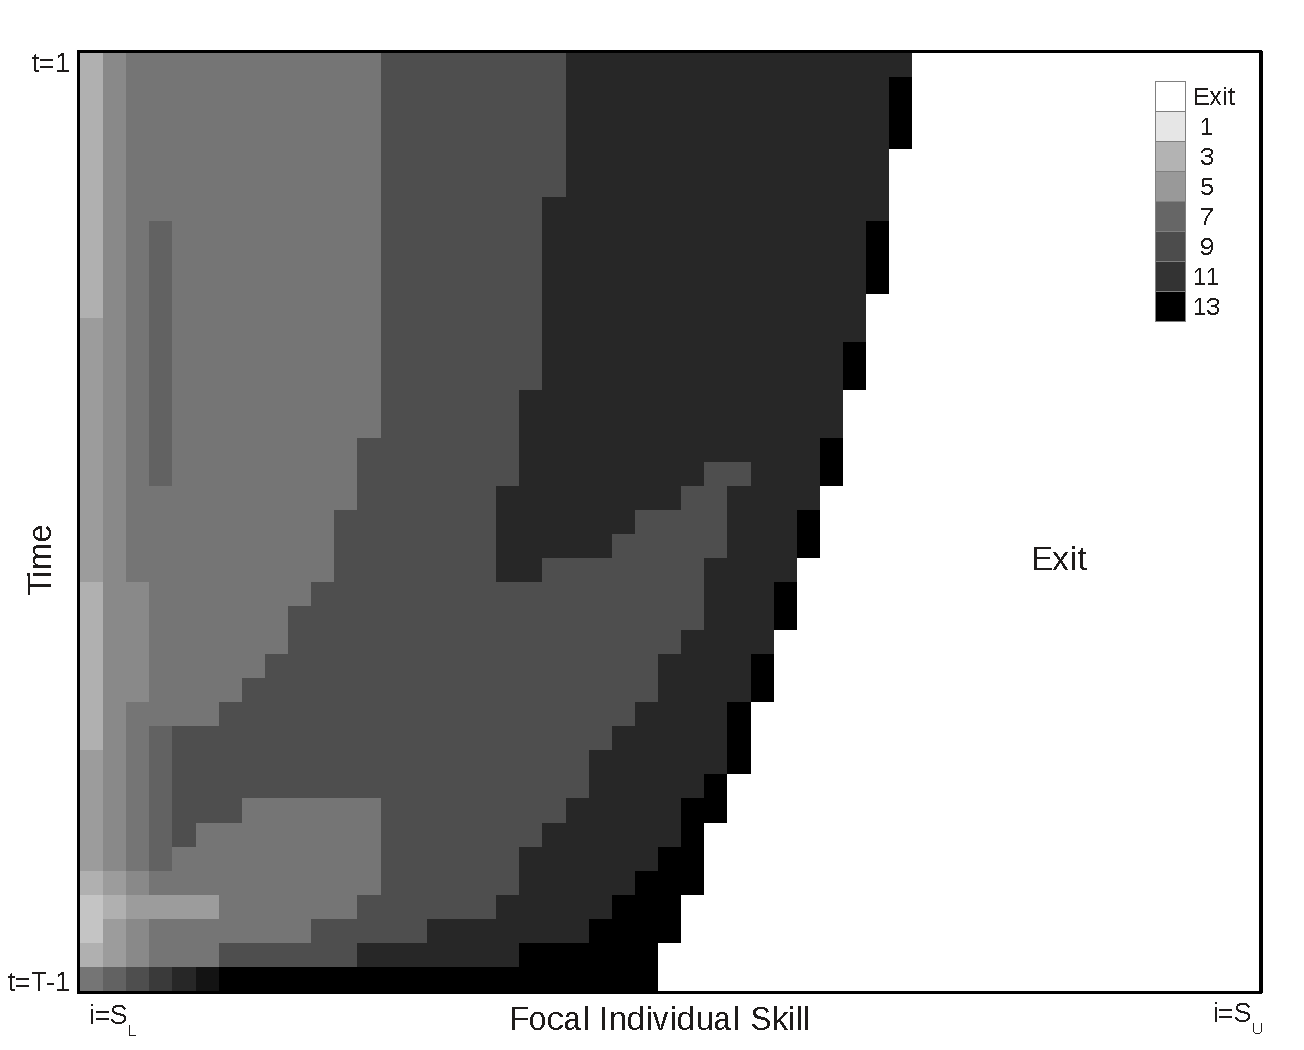
\includegraphics[width=170mm]{TplayHeat.pdf}
%\label{map}
%\caption{stay model}
%\includegraphics[width=150mm]{playOpportunitesExit.png}\\
%\includegraphics[width=150mm]{playOpportunitesExitBold.png}
\end{center}
\label{mapExit}
\end{figure}



%fitness at time
\begin{figure}[h]
\begin{center}
\caption{$F(i,t)$. The focal individual fitness plotted against skill level. Each line is a single time period of the model. Three time periods of the model are plotted. Notice when many time periods remain in the model, fitness is relatively high for all skill levels, due to the prospect of gaining skill in the future. As the number of periods remaining in the model decreases, the fitness of low skill individuals decreases due to reduced prospect for the future. Additionally, the dotted vertical lines mark the skill at which $F(i,t)$ converges with $\phi(i)$. These dotted lines mark the skill at which the focal individual stops considering play behavior at the given time period of the model. Notice that with many time periods of the model remaining only very high skill individuals exit the model, and as the number of time periods remaining in the model decreases this exit skill decreases.  }
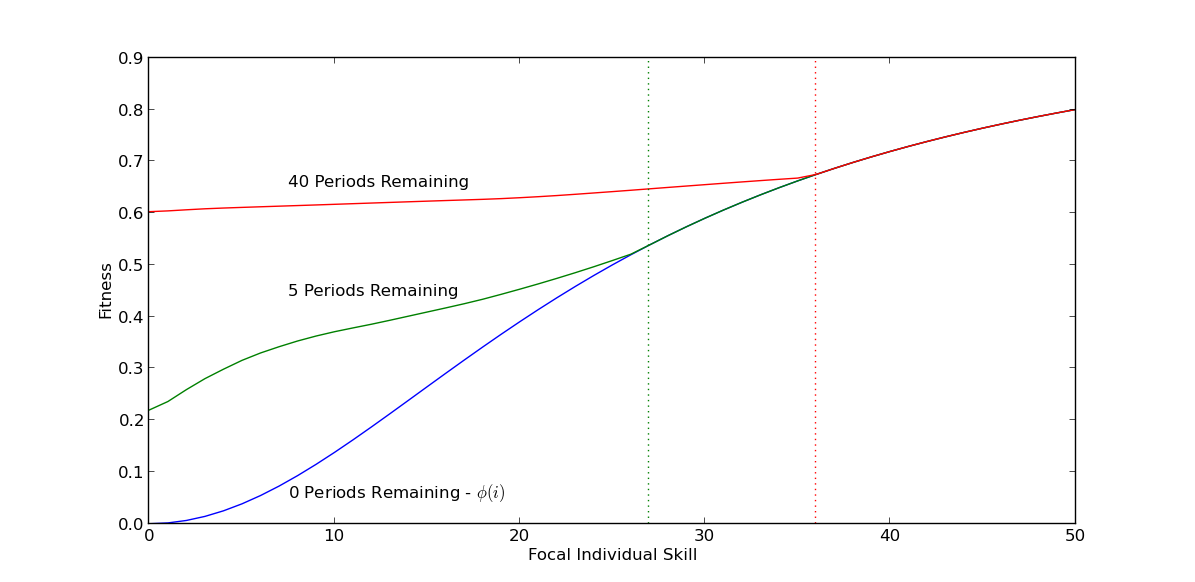
\includegraphics[width=160mm]{fitness.png}
\end{center}
\label{fit}
\end{figure}



\end{figure}
\begin{figure}
\caption{Final skill distribution of $k=250$ Monte Carlo simulated individuals. Each individuals starts the simulation with a uniform random skill level on the interval $[S_L,S_U]$. Each individual makes optimal decisions, based on $D^*(i,j,t)$, for 40 time periods. Notice the bimodal distribution of the final skills. }
\begin{center}
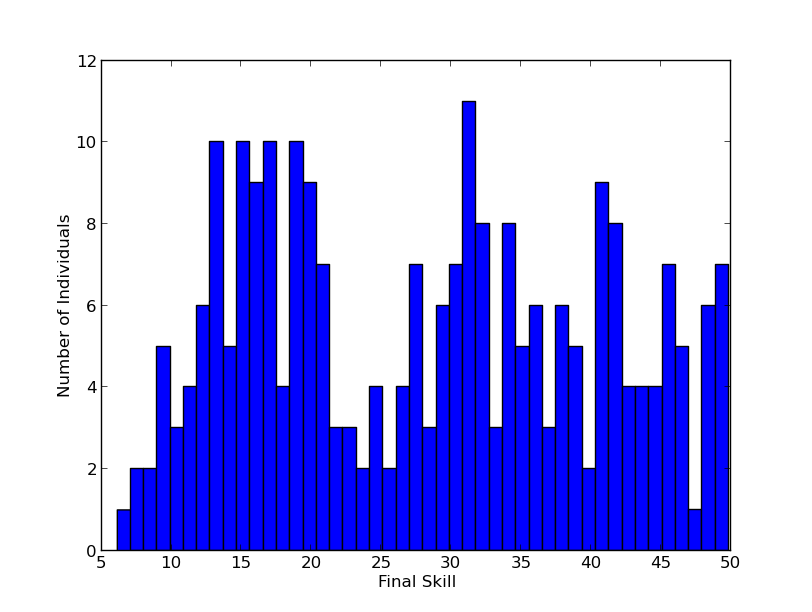
\includegraphics[width=150mm]{Fmcmc.png}
\end{center}
\label{Fmcmc}
\end{figure}



%scatter
\begin{figure}[h]
\caption{Final skill distribution of $k=250$ Monte Carlo simulated individuals plotted against the initial skill distribution. The red dotted line indicates the one-to-one relationship between initial and final skill. Individuals on the one-to-one line, in the region labeled ``Exit", enter the simulation with high enough skills to immediately exit play behavior. Notice for each initial skill below the initial exit skill, the final skill distributions are very similar, both to each other, and to the final skill distribution seen in Figure 7. }
\begin{center}
%\includegraphics[width=150mm]{mcmc.png}
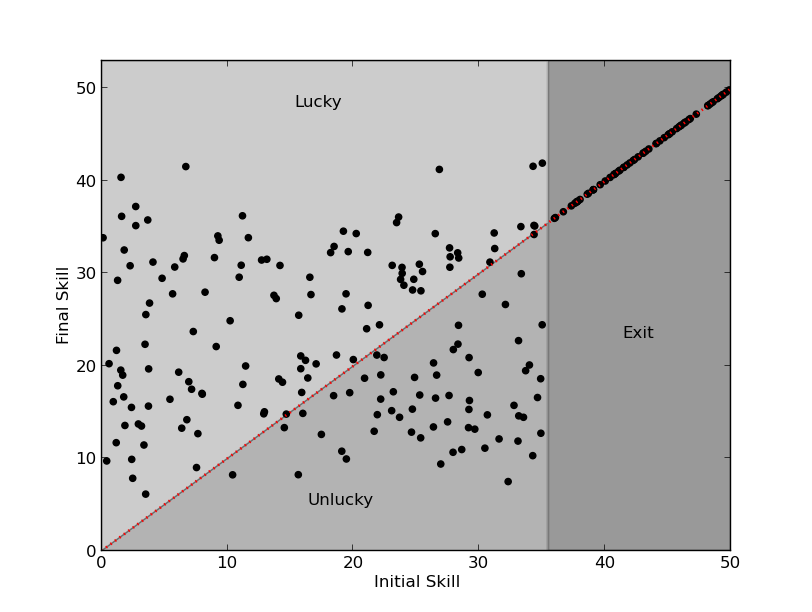
\includegraphics[width=150mm]{mcmc2.png}
\end{center}
\label{mcmc}
\end{figure}

